\textit{Apriori}~\cite{agarwal2001tree} è un algoritmo pensato per affrontare il problema della generazione
e filtraggio dei candidati in maniera efficace e efficiente.
Apriori utilizza una struttura di generazione a livelli in maniera iterativa: ad ogni livello sono ricercati pattern di dimensioni \(k\)
aventi supporto maggiore di \(minsupp\).
Successivamente i pattern validi sono impiegati nella costruzione
del livello successivo, mentre gli altri sono scartati.
Intuitivamente, la ragione per cui accade ciò è che la frequenza di un set sarà sempre maggiore di
quella di qualunque superset a cui questo appartiene.Se già un set non soddisfa il vincolo di frequenza,
nessun suo superset potrà fare altrettanto.
Questo principio è noto con il nome di monotonicità della generazione apriori.
Ne segue che tutti gli itemset generati al livello \(k + 1\) saranno combinazioni di pattern validi al livello
\(k\).
Questa strategia di generazione permette di scartare un grande numero di itemset e le loro successive
combinazioni (\cref{fig:chap-1:apriori-example}).

\begin{figure}
\centering
  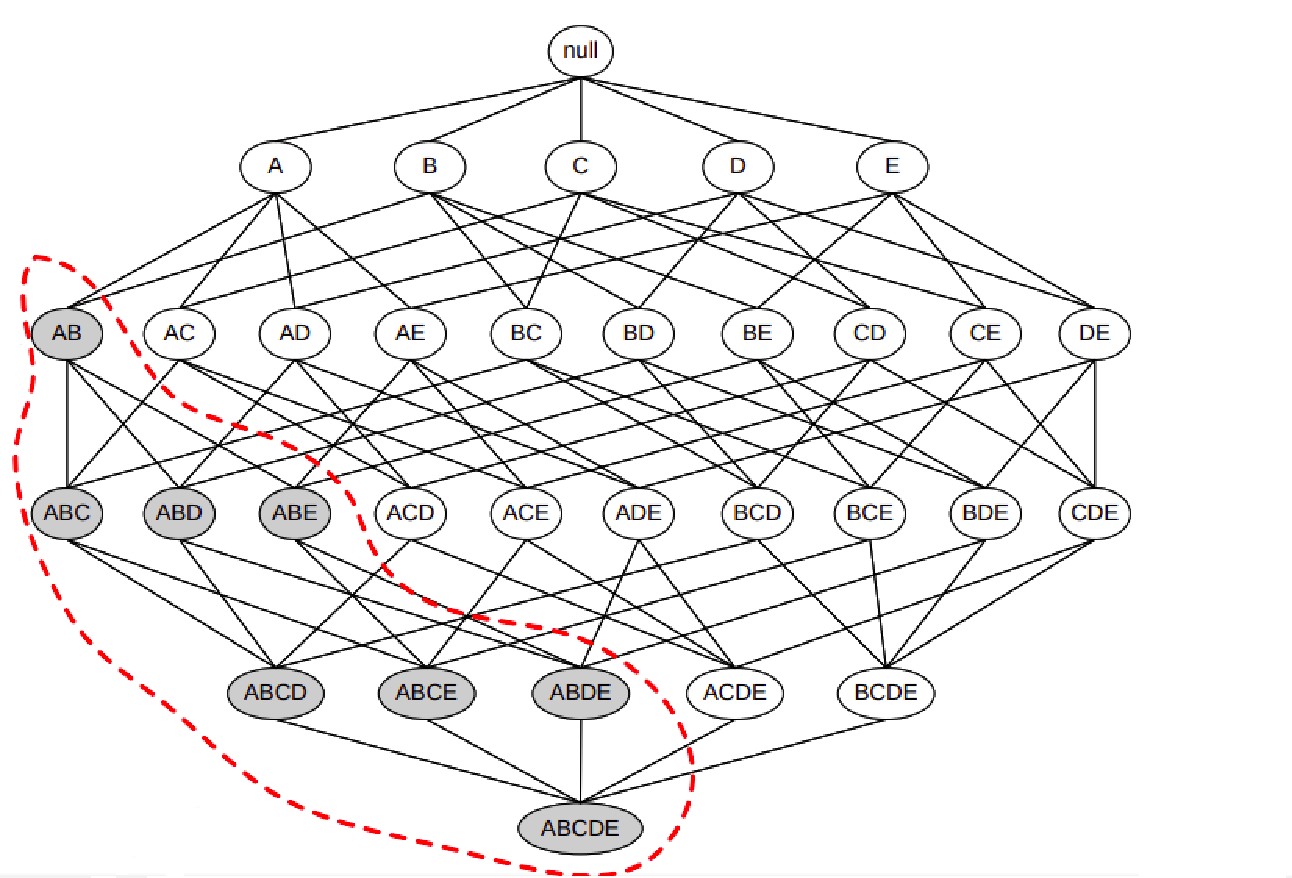
\includegraphics[width=\textwidth]{/sec-1/APrioriExample.pdf}
  \caption{Esempio di struttura gerarchica generata dall'algoritmo Apriori, in questo caso l'itemset \( \{ a,b \} \) non risulta frequente, di conseguenza i suoi superset sono scartati,Fonte:~\cite{biascsru72:online}}%
  \label{fig:chap-1:apriori-example}
\end{figure}

All'interno dell'insieme degli itemset validi, è possibile eseguire un'ulteriore distinzione:
si definiscono chiusi (\textit{closed}) gli itemset aventi supporto strettamente maggiore di
tutti i propri superset (\cref{definition:closed-itemset}); al contrario un itemset non avente superset validi è definibile come
massimale (\cref{definition:maximal-itemset}).

\begin{definition}[Itemset chiuso]\label{definition:closed-itemset}
L'itemset \(I\) si definisce chiuso se \( \forall J~\text{t.c}~ I \subset J,~ s(I) > s(J)\)
\end{definition}

\begin{definition}[Itemset massimale]\label{definition:maximal-itemset}
L'itemset \(I\) si definisce massimale se \( \forall J~\text{t.c}~ I \subset J,~s(J) < minsup\)
\end{definition}

\begin{figure}
\centering
  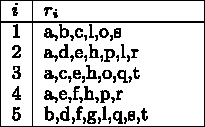
\includegraphics[width=0.5\textwidth]{res/fig/sec-1/TransactionSetExample.pdf}
  \caption{Dataset contenente 5 transazioni, fissato \(minsup = 2\) l'itemset \((a,e,h)\) risulta chiuso e massimale, Fonte:~\cite{pan2003carpenter}}%
  \label{fig:chap-1:dataset-example}
\end{figure}

Preso come esempio il dataset in \cref{fig:chap-1:dataset-example}, il pattern \((a,e,h)\) risulta chiuso, in quanto nessuno dei suoi superset ha un supporto maggiore del suo.
\((a,e,h)\) inoltre può essere definito anche come pattern massimale, in quanto tutti i suoi superset hanno supporto minore di \(minsup\).
L'itemset \((a,e)\) invece risulta frequente, ma né chiuso né massimale, in quanto \(s((a,e)) = s((a,e,h))\).

L'esempio sopra mostra un'altra proprietà di chiusura e massimalità: ogni pattern massimale, come nell'esempio, può essere categorizzato come pattern chiuso.
Un pattern massimale è infatti un itemset frequente i cui superset hanno supporto minore di \(minsup\), tuttavia per definizione di frequenza \(s(pattern) \geq minsup\).
Ne segue che sarà sempre vero che il pattern in questione avrà supporto maggiore di tutti i suoi superset, rientrando così nella definizione di massimale.
Al contrario non tutti pattern chiusi possono essere classificati come massimali.
Non c'è infatti nessuna proprietà che garantisca che un superset di un itemset abbia una frequenza minore dell'itemset stesso, come ad esempio succede nel caso sopracitato.


In molti casi Apriori è efficace nel ridurre lo spazio di ricerca di itemset validi, tuttavia
soffre di alcuni limiti: in primo luogo è molto probabile che il numero di candidati generati rimanga comunque
alto, in quanto molti di questi sono generati in un primo momento e scartati dopo il calcolo del supporto.
Proprio a quest'ultimo punto si collega un'altra problematica: la computazione del supporto richiede molte
scansioni delle transazioni e ad ogni livello devono essere verificati molti itemset.
Prendendo ad esempio il dataset in \cref{fig:chap-1:dataset-example}, in cui sono presenti solo 5 righe e 15 item, sono generate e valutate tutte le combinazioni di item.
Questo implica la valutazione di \(2^15\) possibili itemset.
Ovviamente questo numero cala specificando soglie di supporto con valori alti.
Tuttavia è probabile che soprattutto nei primi passi, il numero di itemset individuati esploda, peggiorando di conseguenza le performance dell'algoritmo.
